\documentclass[conference]{IEEEtran}
\IEEEoverridecommandlockouts
\usepackage{cite}
\usepackage{amsmath,amssymb,amsfonts}
\usepackage{graphicx}
\usepackage{textcomp}
\usepackage{xcolor}
\usepackage{booktabs}
\usepackage{multirow}
\usepackage{url}
\usepackage[hidelinks]{hyperref}
% AUTO-GENERATED by phishresearch.reporting - do not edit
\makeatletter
\newcommand{\res}[1]{\@ifundefined{r@#1}{\textbf{??#1??}}{\@nameuse{r@#1}}}
\@namedef{r@freezeHash}{069912e332d7}
\@namedef{r@nBoot}{2,000}
\@namedef{r@nAn}{73,575}
\@namedef{r@cAn}{46,769}
\@namedef{r@nAbenign}{36,400}
\@namedef{r@cAbenign}{22,167}
\@namedef{r@nAphishing}{37,175}
\@namedef{r@cAphishing}{24,602}
\@namedef{r@dupA}{18,811}
\@namedef{r@quarA}{3}
\@namedef{r@purgeA}{7,992}
\@namedef{r@lossBenignA}{25.9}
\@namedef{r@lossPhishA}{1.0}
\@namedef{r@groupsA}{20,913}
\@namedef{r@topGroupA}{esy.es}
\@namedef{r@topGroupShareA}{2.9}
\@namedef{r@nBn}{92,500}
\@namedef{r@cBn}{75,077}
\@namedef{r@nBbenign}{46,250}
\@namedef{r@cBbenign}{29,758}
\@namedef{r@nBphishing}{46,250}
\@namedef{r@cBphishing}{45,319}
\@namedef{r@dupB}{1}
\@namedef{r@quarB}{17}
\@namedef{r@purgeB}{17,405}
\@namedef{r@lossBenignB}{35.6}
\@namedef{r@lossPhishB}{2.0}
\@namedef{r@groupsB}{6,735}
\@namedef{r@topGroupB}{esnafbenim.com}
\@namedef{r@topGroupShareB}{11.0}
\@namedef{r@sharedGroups}{692}
\@namedef{r@exactOverlap}{33}
\@namedef{r@labelJoin}{73,575}
\@namedef{r@labelAgree}{100.0}
\@namedef{r@splitAFIT}{28,061}
\@namedef{r@splitGroupsAFIT}{8,018}
\@namedef{r@splitAVAL}{9,355}
\@namedef{r@splitGroupsAVAL}{6,448}
\@namedef{r@splitATEST}{9,353}
\@namedef{r@splitGroupsATEST}{6,447}
\@namedef{r@splitBFIT}{45,050}
\@namedef{r@splitGroupsBFIT}{2,614}
\@namedef{r@splitBVAL}{15,014}
\@namedef{r@splitGroupsBVAL}{2,060}
\@namedef{r@splitBTEST}{15,013}
\@namedef{r@splitGroupsBTEST}{2,061}
\@namedef{r@F1AARFALL}{0.895}
\@namedef{r@F1loAARFALL}{0.887}
\@namedef{r@F1hiAARFALL}{0.902}
\@namedef{r@APAARFALL}{0.962}
\@namedef{r@RecAARFALL}{0.475}
\@namedef{r@FPRAARFALL}{0.7}
\@namedef{r@F1dbAARFALL}{0.862}
\@namedef{r@F1AARFMEANPIbudget}{0.897}
\@namedef{r@F1loAARFMEANPIbudget}{0.889}
\@namedef{r@F1hiAARFMEANPIbudget}{0.904}
\@namedef{r@APAARFMEANPIbudget}{0.962}
\@namedef{r@RecAARFMEANPIbudget}{0.478}
\@namedef{r@FPRAARFMEANPIbudget}{0.8}
\@namedef{r@F1dbAARFMEANPIbudget}{0.865}
\@namedef{r@F1AARFSTABLEPIbudget}{0.896}
\@namedef{r@F1loAARFSTABLEPIbudget}{0.889}
\@namedef{r@F1hiAARFSTABLEPIbudget}{0.903}
\@namedef{r@APAARFSTABLEPIbudget}{0.962}
\@namedef{r@RecAARFSTABLEPIbudget}{0.468}
\@namedef{r@FPRAARFSTABLEPIbudget}{0.7}
\@namedef{r@F1dbAARFSTABLEPIbudget}{0.864}
\@namedef{r@F1AALGBMALL}{0.902}
\@namedef{r@F1loAALGBMALL}{0.894}
\@namedef{r@F1hiAALGBMALL}{0.909}
\@namedef{r@APAALGBMALL}{0.966}
\@namedef{r@RecAALGBMALL}{0.559}
\@namedef{r@FPRAALGBMALL}{0.9}
\@namedef{r@F1dbAALGBMALL}{0.872}
\@namedef{r@F1AALGBMMEANPIbudget}{0.900}
\@namedef{r@F1loAALGBMMEANPIbudget}{0.893}
\@namedef{r@F1hiAALGBMMEANPIbudget}{0.908}
\@namedef{r@APAALGBMMEANPIbudget}{0.965}
\@namedef{r@RecAALGBMMEANPIbudget}{0.553}
\@namedef{r@FPRAALGBMMEANPIbudget}{1.0}
\@namedef{r@F1dbAALGBMMEANPIbudget}{0.873}
\@namedef{r@F1AALGBMSTABLEPIbudget}{0.900}
\@namedef{r@F1loAALGBMSTABLEPIbudget}{0.892}
\@namedef{r@F1hiAALGBMSTABLEPIbudget}{0.907}
\@namedef{r@APAALGBMSTABLEPIbudget}{0.965}
\@namedef{r@RecAALGBMSTABLEPIbudget}{0.549}
\@namedef{r@FPRAALGBMSTABLEPIbudget}{1.0}
\@namedef{r@F1dbAALGBMSTABLEPIbudget}{0.873}
\@namedef{r@F1ABRFALL}{0.917}
\@namedef{r@F1loABRFALL}{0.905}
\@namedef{r@F1hiABRFALL}{0.929}
\@namedef{r@APABRFALL}{0.947}
\@namedef{r@RecABRFALL}{0.017}
\@namedef{r@FPRABRFALL}{0.3}
\@namedef{r@F1dbABRFALL}{0.782}
\@namedef{r@F1ABRFMEANPIbudget}{0.914}
\@namedef{r@F1loABRFMEANPIbudget}{0.901}
\@namedef{r@F1hiABRFMEANPIbudget}{0.925}
\@namedef{r@APABRFMEANPIbudget}{0.947}
\@namedef{r@RecABRFMEANPIbudget}{0.017}
\@namedef{r@FPRABRFMEANPIbudget}{0.3}
\@namedef{r@F1dbABRFMEANPIbudget}{0.767}
\@namedef{r@F1ABRFSTABLEPIbudget}{0.913}
\@namedef{r@F1loABRFSTABLEPIbudget}{0.901}
\@namedef{r@F1hiABRFSTABLEPIbudget}{0.924}
\@namedef{r@APABRFSTABLEPIbudget}{0.950}
\@namedef{r@RecABRFSTABLEPIbudget}{0.016}
\@namedef{r@FPRABRFSTABLEPIbudget}{0.2}
\@namedef{r@F1dbABRFSTABLEPIbudget}{0.763}
\@namedef{r@F1ABLGBMALL}{0.922}
\@namedef{r@F1loABLGBMALL}{0.910}
\@namedef{r@F1hiABLGBMALL}{0.933}
\@namedef{r@APABLGBMALL}{0.958}
\@namedef{r@RecABLGBMALL}{0.345}
\@namedef{r@FPRABLGBMALL}{1.6}
\@namedef{r@F1dbABLGBMALL}{0.796}
\@namedef{r@F1ABLGBMMEANPIbudget}{0.916}
\@namedef{r@F1loABLGBMMEANPIbudget}{0.903}
\@namedef{r@F1hiABLGBMMEANPIbudget}{0.927}
\@namedef{r@APABLGBMMEANPIbudget}{0.956}
\@namedef{r@RecABLGBMMEANPIbudget}{0.510}
\@namedef{r@FPRABLGBMMEANPIbudget}{1.8}
\@namedef{r@F1dbABLGBMMEANPIbudget}{0.778}
\@namedef{r@F1ABLGBMSTABLEPIbudget}{0.915}
\@namedef{r@F1loABLGBMSTABLEPIbudget}{0.902}
\@namedef{r@F1hiABLGBMSTABLEPIbudget}{0.927}
\@namedef{r@APABLGBMSTABLEPIbudget}{0.956}
\@namedef{r@RecABLGBMSTABLEPIbudget}{0.482}
\@namedef{r@FPRABLGBMSTABLEPIbudget}{1.7}
\@namedef{r@F1dbABLGBMSTABLEPIbudget}{0.776}
\@namedef{r@F1BBRFALL}{0.956}
\@namedef{r@F1loBBRFALL}{0.947}
\@namedef{r@F1hiBBRFALL}{0.964}
\@namedef{r@APBBRFALL}{0.993}
\@namedef{r@RecBBRFALL}{0.831}
\@namedef{r@FPRBBRFALL}{0.4}
\@namedef{r@F1dbBBRFALL}{0.916}
\@namedef{r@F1BBRFMEANPIbudget}{0.941}
\@namedef{r@F1loBBRFMEANPIbudget}{0.930}
\@namedef{r@F1hiBBRFMEANPIbudget}{0.950}
\@namedef{r@APBBRFMEANPIbudget}{0.989}
\@namedef{r@RecBBRFMEANPIbudget}{0.823}
\@namedef{r@FPRBBRFMEANPIbudget}{0.6}
\@namedef{r@F1dbBBRFMEANPIbudget}{0.888}
\@namedef{r@F1BBRFSTABLEPIbudget}{0.944}
\@namedef{r@F1loBBRFSTABLEPIbudget}{0.933}
\@namedef{r@F1hiBBRFSTABLEPIbudget}{0.953}
\@namedef{r@APBBRFSTABLEPIbudget}{0.989}
\@namedef{r@RecBBRFSTABLEPIbudget}{0.820}
\@namedef{r@FPRBBRFSTABLEPIbudget}{0.8}
\@namedef{r@F1dbBBRFSTABLEPIbudget}{0.904}
\@namedef{r@F1BBLGBMALL}{0.958}
\@namedef{r@F1loBBLGBMALL}{0.949}
\@namedef{r@F1hiBBLGBMALL}{0.966}
\@namedef{r@APBBLGBMALL}{0.993}
\@namedef{r@RecBBLGBMALL}{0.876}
\@namedef{r@FPRBBLGBMALL}{0.5}
\@namedef{r@F1dbBBLGBMALL}{0.936}
\@namedef{r@F1BBLGBMMEANPIbudget}{0.942}
\@namedef{r@F1loBBLGBMMEANPIbudget}{0.932}
\@namedef{r@F1hiBBLGBMMEANPIbudget}{0.951}
\@namedef{r@APBBLGBMMEANPIbudget}{0.990}
\@namedef{r@RecBBLGBMMEANPIbudget}{0.820}
\@namedef{r@FPRBBLGBMMEANPIbudget}{0.2}
\@namedef{r@F1dbBBLGBMMEANPIbudget}{0.871}
\@namedef{r@F1BBLGBMSTABLEPIbudget}{0.946}
\@namedef{r@F1loBBLGBMSTABLEPIbudget}{0.937}
\@namedef{r@F1hiBBLGBMSTABLEPIbudget}{0.955}
\@namedef{r@APBBLGBMSTABLEPIbudget}{0.990}
\@namedef{r@RecBBLGBMSTABLEPIbudget}{0.821}
\@namedef{r@FPRBBLGBMSTABLEPIbudget}{0.3}
\@namedef{r@F1dbBBLGBMSTABLEPIbudget}{0.895}
\@namedef{r@F1BARFALL}{0.739}
\@namedef{r@F1loBARFALL}{0.727}
\@namedef{r@F1hiBARFALL}{0.751}
\@namedef{r@APBARFALL}{0.829}
\@namedef{r@RecBARFALL}{0.115}
\@namedef{r@FPRBARFALL}{1.4}
\@namedef{r@F1dbBARFALL}{0.703}
\@namedef{r@F1BARFMEANPIbudget}{0.639}
\@namedef{r@F1loBARFMEANPIbudget}{0.625}
\@namedef{r@F1hiBARFMEANPIbudget}{0.652}
\@namedef{r@APBARFMEANPIbudget}{0.739}
\@namedef{r@RecBARFMEANPIbudget}{0.101}
\@namedef{r@FPRBARFMEANPIbudget}{2.2}
\@namedef{r@F1dbBARFMEANPIbudget}{0.604}
\@namedef{r@F1BARFSTABLEPIbudget}{0.697}
\@namedef{r@F1loBARFSTABLEPIbudget}{0.685}
\@namedef{r@F1hiBARFSTABLEPIbudget}{0.710}
\@namedef{r@APBARFSTABLEPIbudget}{0.746}
\@namedef{r@RecBARFSTABLEPIbudget}{0.135}
\@namedef{r@FPRBARFSTABLEPIbudget}{3.1}
\@namedef{r@F1dbBARFSTABLEPIbudget}{0.649}
\@namedef{r@F1BALGBMALL}{0.790}
\@namedef{r@F1loBALGBMALL}{0.779}
\@namedef{r@F1hiBALGBMALL}{0.800}
\@namedef{r@APBALGBMALL}{0.883}
\@namedef{r@RecBALGBMALL}{0.440}
\@namedef{r@FPRBALGBMALL}{3.2}
\@namedef{r@F1dbBALGBMALL}{0.747}
\@namedef{r@F1BALGBMMEANPIbudget}{0.619}
\@namedef{r@F1loBALGBMMEANPIbudget}{0.605}
\@namedef{r@F1hiBALGBMMEANPIbudget}{0.634}
\@namedef{r@APBALGBMMEANPIbudget}{0.772}
\@namedef{r@RecBALGBMMEANPIbudget}{0.143}
\@namedef{r@FPRBALGBMMEANPIbudget}{0.9}
\@namedef{r@F1dbBALGBMMEANPIbudget}{0.588}
\@namedef{r@F1BALGBMSTABLEPIbudget}{0.697}
\@namedef{r@F1loBALGBMSTABLEPIbudget}{0.685}
\@namedef{r@F1hiBALGBMSTABLEPIbudget}{0.709}
\@namedef{r@APBALGBMSTABLEPIbudget}{0.790}
\@namedef{r@RecBALGBMSTABLEPIbudget}{0.220}
\@namedef{r@FPRBALGBMSTABLEPIbudget}{2.2}
\@namedef{r@F1dbBALGBMSTABLEPIbudget}{0.653}
\@namedef{r@DropALGBMALL}{-2.0}
\@namedef{r@DropALGBMMEANPIbudget}{-1.5}
\@namedef{r@DropALGBMMEANPImatched}{-1.5}
\@namedef{r@DropALGBMSTABLEPIbudget}{-1.6}
\@namedef{r@DropALGBMSTABLEPImatched}{-1.6}
\@namedef{r@DropARFALL}{-2.3}
\@namedef{r@DropARFMEANPIbudget}{-1.7}
\@namedef{r@DropARFMEANPImatched}{-1.7}
\@namedef{r@DropARFSTABLEPIbudget}{-1.7}
\@namedef{r@DropARFSTABLEPImatched}{-1.7}
\@namedef{r@DropBLGBMALL}{16.9}
\@namedef{r@DropBLGBMMEANPIbudget}{32.3}
\@namedef{r@DropBLGBMMEANPImatched}{32.3}
\@namedef{r@DropBLGBMSTABLEPIbudget}{25.0}
\@namedef{r@DropBLGBMSTABLEPImatched}{25.0}
\@namedef{r@DropBRFALL}{21.7}
\@namedef{r@DropBRFMEANPIbudget}{30.2}
\@namedef{r@DropBRFMEANPImatched}{30.2}
\@namedef{r@DropBRFSTABLEPIbudget}{24.7}
\@namedef{r@DropBRFSTABLEPImatched}{24.7}
\@namedef{r@DropMin}{-2.3}
\@namedef{r@DropMax}{21.7}
\@namedef{r@DeltaABRF}{-0.000}
\@namedef{r@DeltaLoABRF}{-0.001}
\@namedef{r@DeltaHiABRF}{+0.000}
\@namedef{r@DeltaABLGBM}{-0.000}
\@namedef{r@DeltaLoABLGBM}{-0.001}
\@namedef{r@DeltaHiABLGBM}{+0.000}
\@namedef{r@DeltaBARF}{+0.059}
\@namedef{r@DeltaLoBARF}{+0.051}
\@namedef{r@DeltaHiBARF}{+0.066}
\@namedef{r@DeltaBALGBM}{+0.077}
\@namedef{r@DeltaLoBALGBM}{+0.069}
\@namedef{r@DeltaHiBALGBM}{+0.086}
\@namedef{r@nPrimaryExcl}{2}
\@namedef{r@nPrimaryPos}{2}
\@namedef{r@nPrimaryEff}{2}
\@namedef{r@SecABRFSTABLEALL}{-0.004}
\@namedef{r@SecABRFMEANALL}{-0.004}
\@namedef{r@SecABRFSTABLE}{-0.000}
\@namedef{r@SecABLGBMSTABLEALL}{-0.007}
\@namedef{r@SecABLGBMMEANALL}{-0.006}
\@namedef{r@SecABLGBMSTABLE}{-0.000}
\@namedef{r@SecBARFSTABLEALL}{-0.042}
\@namedef{r@SecBARFMEANALL}{-0.100}
\@namedef{r@SecBARFSTABLE}{+0.059}
\@namedef{r@SecBALGBMSTABLEALL}{-0.093}
\@namedef{r@SecBALGBMMEANALL}{-0.170}
\@namedef{r@SecBALGBMSTABLE}{+0.077}
\@namedef{r@highCorrA}{14}
\@namedef{r@piSecA}{26.1}
\@namedef{r@highCorrB}{17}
\@namedef{r@piSecB}{10.6}
\@namedef{r@relLatB1Min}{0.75}
\@namedef{r@relLatB1Max}{1.10}
\@namedef{r@relLatBkMin}{0.47}
\@namedef{r@relLatBkMax}{1.01}
\@namedef{r@extractShareMedian}{10.4}
\@namedef{r@cpu}{Intel64 Family 6 Model 154 Stepping 3, GenuineIntel}
\@namedef{r@ram}{32}
\@namedef{r@pyver}{3.10.0}
\@namedef{r@RhoALGBMALL}{0.99}
\@namedef{r@RhoALGBMSTABLEPIbudget}{0.88}
\@namedef{r@RhoARFALL}{0.97}
\@namedef{r@RhoARFSTABLEPIbudget}{0.81}
\@namedef{r@RhoBLGBMALL}{0.96}
\@namedef{r@RhoBLGBMSTABLEPIbudget}{0.98}
\@namedef{r@RhoBRFALL}{0.95}
\@namedef{r@RhoBRFSTABLEPIbudget}{0.98}
\@namedef{r@shapAddErr}{3.3e-03}
\@namedef{r@rhoMin}{0.81}
\@namedef{r@rhoMax}{0.99}
\@namedef{r@rhoSeedMin}{1.00}
\@namedef{r@medLenABenign}{55}
\@namedef{r@medDotsABenign}{2}
\@namedef{r@medSubABenign}{1}
\@namedef{r@httpsABenign}{34.9}
\@namedef{r@medLenAPhish}{63}
\@namedef{r@medDotsAPhish}{2}
\@namedef{r@medSubAPhish}{0}
\@namedef{r@httpsAPhish}{1.5}
\@namedef{r@medLenBBenign}{41}
\@namedef{r@medDotsBBenign}{2}
\@namedef{r@medSubBBenign}{1}
\@namedef{r@httpsBBenign}{83.5}
\@namedef{r@medLenBPhish}{74}
\@namedef{r@medDotsBPhish}{5}
\@namedef{r@medSubBPhish}{3}
\@namedef{r@httpsBPhish}{30.6}
\@namedef{r@status}{benchmark: completed, evaluation: completed, shap: completed}
\makeatother

\newcommand{\EBBU}{EBBU}
\newcommand{\HP}{HP}

\begin{document}

\title{Source-Only Feature Selection for Lightweight Phishing URL Detection with Bidirectional Cross-Dataset Evaluation}

\author{\IEEEauthorblockN{[Author Name]}
\IEEEauthorblockA{\textit{[Department]} \\
\textit{[Affiliation]}\\
[City, Country] \\
[email]}
}

\maketitle

\begin{abstract}
Cross-dataset phishing detection is already studied, but feature reduction must also be assessed when target observations are unavailable for learning and calibration. We evaluate whether source-domain feature stability improves transfer over mean importance at equal feature budgets, and whether it reduces detection cost. EBBU-2017 and HISPAR--Phishstats (HP) form a curated benchmark with symmetric shared-domain purge and domain-disjoint splits. Random forest and LightGBM use offline lexical features, nested source-only budget selection and source-validation thresholds, with a frozen experimental protocol. Transfer is asymmetric: EBBU-trained LightGBM reaches F1 \res{F1ABLGBMALL} on HP, whereas HP-trained models reach \res{F1BARFALL}--\res{F1BALGBMALL} on EBBU. At equal budgets, stability ranking improves HP$\rightarrow$EBBU F1 over mean ranking by \res{DeltaBARF} (RF) and \res{DeltaBALGBM} (LightGBM), but shows no clear advantage in the opposite direction. Reduced subsets do not match the full feature set across datasets, and latency benefits depend on the model and execution setting. The contribution is an auditable empirical comparison and a bounded transfer--cost insight, not a new learning algorithm or evidence of superiority over domain adaptation.
\end{abstract}


\begin{IEEEkeywords}
phishing detection, URL classification, cross-dataset evaluation, feature selection, permutation importance, LightGBM, random forest, domain-disjoint split
\end{IEEEkeywords}

\section{Introduction}
Lexical URL classifiers are attractive for phishing defence because they need only the URL string: no page fetch, DNS lookup or third-party reputation service, which keeps them cheap and usable before a user clicks. Such classifiers routinely report near-ceiling accuracy when trained and tested on random splits of one dataset~\cite{sahingoz2019}. That number answers a narrow question. A deployed detector meets URLs collected by a different process, at a different time and from different hosting ecosystems, and recent work shows that lexical models trained on one public corpus lose much of their accuracy on another~\cite{rashid2024,kanon2026,misiek2026}. In a security setting the failure mode matters: a model that transfers poorly either misses phishing or floods analysts with false alarms on benign sites it has never seen.

Two remedies are common. Domain adaptation uses (unlabelled) target data to align the source and target distributions~\cite{rashid2024}. Cross-dataset feature selection keeps only features that are important on several datasets~\cite{kanon2026,misiek2026}. Both consult the target distribution before evaluation, so a reported gain partly reflects access to the very population on which the model is scored. In addition, URL-level random splits let URLs of the same registered domain fall on both sides of the train/test boundary, which rewards memorising domains rather than learning transferable cues.

This paper studies the stricter \emph{source-only} question: when nothing about the target is available, does choosing features by the \emph{stability} of their importance across held-out domains of the source improve transfer, and does a smaller feature set reduce cost? We make three contributions, which we frame as a carefully controlled empirical study rather than a new algorithm.
\begin{enumerate}
\item A curated, \emph{domain-disjoint} benchmark built from two public sources, EBBU-2017~\cite{sahingoz2019} and HISPAR--Phishstats (HP)~\cite{rashid2024}: registered domains shared by the two sources are removed symmetrically, and every split is group-disjoint by registered domain.
\item A transparent comparison of two source-only selectors built on the same permutation-importance (PI) evidence---ranking by mean PI (MEAN-PI) or by cross-fold stability (STABLE-PI)---at matched feature budgets, for random forest (RF)~\cite{breiman2001} and LightGBM~\cite{ke2017}, in both transfer directions, with nested selection, thresholds locked on source validation data and domain-cluster bootstrap intervals.
\item A measured account of what feature reduction buys at inference time (end-to-end latency, separated into parsing, feature extraction and prediction) and of how the models' SHAP attributions shift between source and target.
\end{enumerate}
The protocol, code and all analysis decisions were frozen and hashed before any test label was read; null and negative findings are reported as obtained.

\section{Related Work}
\textit{Lexical URL detection.} Sahingoz~\textit{et al.}~\cite{sahingoz2019} released the EBBU-2017 corpus and showed that NLP-style URL features with tree ensembles reach high accuracy on that corpus. We reuse its raw URLs only; our 37 features are our own design and we do not attempt to reproduce their numbers.

\textit{Cross-dataset generalisation.} Rashid~\textit{et al.}~\cite{rashid2024} studied the generalisation of phishing URL classifiers across datasets and proposed unsupervised domain adaptation, which uses unlabelled target URLs during training; their public repository distributes EBBU, HP and ISCX files, from which we take HP. Our setting is strictly source-only; we do not replicate their algorithm or their splits. Kanon~\textit{et al.}~\cite{kanon2026} proposed cross-dataset feature stability selection: the intersection of top-$K$ Gini-important features across three datasets, two of which contribute a 15\% labelled sample of the external evaluation sets (pp.~9, 22 of~\cite{kanon2026}); splits are random at URL level. Misiek and Hyla~\cite{misiek2026} selected XGBoost features with criteria computed on importance across all datasets including the external ones and reported training/inference cost. Both studies therefore select features with information from the target population; neither purges shared domains. The closest idea to ours, stability of importance, is thus not new; what differs is \emph{where} stability is measured (held-out domain folds of the source only), the domain-disjoint protocol, the matched-budget contrast and the bidirectional design.

\textit{Selection bias and evaluation.} Feature selection performed outside the cross-validation loop biases error estimates~\cite{ambroise2002,varma2006}; we therefore nest selection inside source-only outer folds. Permutation importance~\cite{altmann2010} is computed on held-out domains and stability is borrowed in spirit from stability selection~\cite{meinshausen2010}. We report average precision rather than a trapezoidal PR-AUC~\cite{davis2006} and explain the actual tree models with TreeExplainer~\cite{lundberg2020}.

\section{Method}
\subsection{Data and cohort construction}
Source A is EBBU-2017 (\res{nAn} URLs: \res{nAbenign} legitimate, \res{nAphishing} phishing; repository \texttt{ebubekirbbr/pdd} at commit \texttt{90b394d}); the class is given by the file name. Source B is HP (\res{nBn} URLs), rebuilt by concatenating the \texttt{hp\_train/valid/test} files of \texttt{fariza25/PhishingURLDetection} at commit \texttt{ff9f1f5}; the original split is kept only as provenance. Because repository B has no codebook, we verified its label convention on its own copy of EBBU: joining it with source A on the raw URL gave \res{labelJoin} matches with \res{labelAgree}\% agreement, confirming 1 = phishing. All file hashes, sizes and observed counts are stored in a manifest; observed counts equal the expected ones.

URLs are canonicalised offline (no network access is possible during extraction): outer whitespace is trimmed; strings with control characters, schemes other than HTTP(S), invalid ports or unparsable hosts are quarantined (\res{quarA} in A, \res{quarB} in B); hosts are lower-cased and IDNA-encoded, while path, query and fragment keep their case and percent-encoding. Exact duplicates (same canonical key and label) are removed within each source (\res{dupA} in A, \res{dupB} in B), and keys with conflicting labels would be quarantined in both sources (none occurred). Each URL is grouped by its registered domain under the ICANN section of a frozen Public Suffix List snapshot; private suffixes are deliberately ignored so that, e.g., all \texttt{blogspot.com} sites form one conservative group. The two sources shared \res{sharedGroups} registered domains (only \res{exactOverlap} exact URLs); all URLs of these domains were removed from \emph{both} sources (\res{purgeA} from A, \res{purgeB} from B). The purge consults target identities only for this audit, never for learning, and costs mostly benign URLs (\res{lossBenignA}\% of A's and \res{lossBenignB}\% of B's benign URLs, versus \res{lossPhishA}\% and \res{lossPhishB}\% of phishing), because popular legitimate platforms appear in both. Table~\ref{tab:attrition} gives the full attrition. The resulting cohorts have \res{cAn} (A) and \res{cBn} (B) URLs over \res{groupsA} and \res{groupsB} domains; the largest group is \texttt{\res{topGroupA}} (\res{topGroupShareA}\%) in A and \texttt{\res{topGroupB}} (\res{topGroupShareB}\%) in B.

\begin{table}[t]
\caption{Cohort attrition (each URL counted once, at the first stage that removed it).}
\label{tab:attrition}
\centering\scriptsize
\begin{tabular}{llrrr}
\toprule
Source & Stage & URLs & Benign & Phishing \\
\midrule
EBBU-2017 & Loaded & 73,575 & 36,400 & 37,175 \\
EBBU-2017 & Parsed & 73,572 & 36,400 & 37,172 \\
EBBU-2017 & Deduplicated & 54,761 & 29,910 & 24,851 \\
EBBU-2017 & Conflicts removed & 54,761 & 29,910 & 24,851 \\
EBBU-2017 & Cohort (shared domains purged) & 46,769 & 22,167 & 24,602 \\
\midrule
HP & Loaded & 92,500 & 46,250 & 46,250 \\
HP & Parsed & 92,483 & 46,233 & 46,250 \\
HP & Deduplicated & 92,482 & 46,233 & 46,249 \\
HP & Conflicts removed & 92,482 & 46,233 & 46,249 \\
HP & Cohort (shared domains purged) & 75,077 & 29,758 & 45,319 \\
\bottomrule
\end{tabular}

\end{table}

\subsection{Splits}
Each source is split into FIT/VAL/TEST ($\approx$60/20/20\% of URLs) by a deterministic greedy stratified \emph{group} assignment (seed 20261115): whole domains are placed, largest first, into the partition whose per-class quota is most unfilled. Partitions share no domain, within or across sources, and keep the class prevalence (Table~\ref{tab:splits}). FIT is used for selection and fitting, VAL only for thresholds, and TEST once, after freezing.

\begin{table}[t]
\caption{Group-disjoint partitions.}
\label{tab:splits}
\centering\scriptsize
\begin{tabular}{llrrrr}
\toprule
Source & Part & URLs & Domains & \% URLs & \% phish \\
\midrule
EBBU & FIT & 28,061 & 8,018 & 60.0 & 52.6 \\
EBBU & VAL & 9,355 & 6,448 & 20.0 & 52.6 \\
EBBU & TEST & 9,353 & 6,447 & 20.0 & 52.6 \\
HP & FIT & 45,050 & 2,614 & 60.0 & 60.4 \\
HP & VAL & 15,014 & 2,060 & 20.0 & 60.4 \\
HP & TEST & 15,013 & 2,061 & 20.0 & 60.4 \\
\bottomrule
\end{tabular}

\end{table}

\subsection{Features}
We use 37 deterministic lexical features (lengths of URL, host, path, query and fragment; counts of 10 delimiter characters, digits, letters and non-ASCII code points; digit ratios; character entropy; longest alphanumeric run; host label and subdomain counts; IP host, explicit port and port number; user-info, query, HTTPS and missing-scheme flags; punycode labels; percent-encoded triplets; query pairs; path segments; and token counts of a fixed 10-word keyword list in the URL and in the host). Raw strings, domains, dataset identity and split labels never enter a model; no vocabulary or target encoding is learned. Each feature is a separate function, so a subset computes only what it needs, while parsing is always paid.

\subsection{Source-only feature selection}
All selectors use the same RF proxy (200 trees, depth 16, min.\ leaf 2, $\sqrt{p}$ features). FIT is divided into three stratified \emph{domain} folds; in each fold the proxy is trained on two folds and the permutation importance (PI) of every feature is measured on the third as the drop in average precision over five permutations. MEAN-PI ranks features by mean PI over the folds. STABLE-PI first counts, for each feature, the folds in which it is in the top $q{=}12$ \emph{and} has PI${>}0$ (votes), then ranks by votes, median PI, the median absolute deviation of its fold ranks, and feature ID. The budget $k\in\{8,16,24\}$ is chosen by nested cross-validation: in three outer domain folds of FIT, PI is recomputed from the outer-training part only, each classifier is trained on the top-$k$ features and scored on the outer hold-out; the smallest $k$ within 0.01 AP of the best mean is kept, separately for every source, classifier, selector and seed. PI is then recomputed on all of FIT for the final subset. To isolate the effect of stability from that of the budget, every STABLE-PI model is paired with a MEAN-PI model at the \emph{same} $k$ (matched-$k$ contrast).

\subsection{Classifiers, thresholds and evaluation}
RF uses 300 trees, depth 20, min.\ leaf 2, $\sqrt{p}$ features; LightGBM uses 300 rounds, learning rate 0.05, 31 leaves, no subsampling, $\lambda_2{=}1$ and deterministic CPU mode. Hyper-parameters are fixed a priori and are not claimed to be optimal~\cite{bergstra2012}. Models are trained on source FIT with seeds 17, 29 and 43. On source VAL we lock (i) the threshold maximising F1 (primary), (ii) the lowest threshold whose VAL false-positive rate is $\le$1\% and (iii) 0.5 (sensitivity). The same model and threshold are then applied to the source TEST (internal) and to the other source's TEST (cross), with no retraining or recalibration on the target. The transfer drop is F1(source TEST)$-$F1(target TEST).

The pre-specified primary outcome is target-TEST F1 of STABLE-PI minus MEAN-PI at matched $k$, for each classifier and direction (four contrasts). Uncertainty is a paired domain-cluster bootstrap (\res{nBoot} replicates): target domains are resampled with replacement, both arms and all three seeds use the same resample, and the per-replicate delta is averaged over seeds. These intervals are conditional on the fixed split and seeds, and we make no family-wise significance claim; an absolute F1 difference of 0.01 was fixed in advance as the smallest difference worth discussing.

\subsection{Cost and attributions}
Latency is measured on the seed-17 model of every configuration with the same interleaved VAL URLs of both sources: 10 warm-up and 300 (batch 1) or 30 (batch 1024) timed repetitions, reporting medians for parsing+feature extraction, prediction alone and end-to-end, with one and with four inference threads. SHAP values are computed with TreeExplainer on the actual classifiers (interventional, probability output, 100 source-FIT background rows) for 500 label-stratified source-TEST and 500 target-TEST URLs, for the seed-17 ALL and STABLE-PI models; additivity against the predicted phishing probability holds to \res{shapAddErr}.

\subsection{Protocol control}
Code, configurations, data splits, feature matrices and all fitted models of both directions were hashed into a freeze manifest (hash \texttt{\res{freezeHash}}) before the evaluator read any TEST label; the development loader cannot load TEST at all. Every number in this paper is generated from the saved predictions and re-computed from them as a check. This is a procedural control rather than a cryptographic guarantee.

\section{Results}
\subsection{Selected budgets}
Nested source-only cross-validation chose $k{=}16$ for every EBBU configuration and $k{=}8$ for every HP configuration, identically for both selectors, both classifiers and all three seeds (Table~\ref{tab:selection}). The matched-$k$ contrast therefore compares two rankings with the same number of input features. Model capacity and tree structure need not be identical, even at equal $k$.

\begin{table}[t]
\caption{Selected budgets ($k$ for seeds 17/29/43) and the STABLE-PI subset of seed 17.}
\label{tab:selection}
\centering\scriptsize
\setlength{\tabcolsep}{4pt}
\begin{tabular}{llccp{3.4cm}}
\toprule
Source & Model & $k$ MEAN & $k$ STABLE & STABLE-PI features (seed 17) \\
\midrule
EBBU & RF & 16/16/16 & 16/16/16 & \scriptsize F02, F03, F04, F06, F07, F08, F09, F16, F18, F21, F22, F23, F24, F30, F35, F36 \\
EBBU & LGBM & 16/16/16 & 16/16/16 & \scriptsize F02, F03, F04, F06, F07, F08, F09, F16, F18, F21, F22, F23, F24, F30, F35, F36 \\
HP & RF & 8/8/8 & 8/8/8 & \scriptsize F02, F03, F06, F21, F22, F23, F24, F30 \\
HP & LGBM & 8/8/8 & 8/8/8 & \scriptsize F02, F03, F06, F21, F22, F23, F24, F30 \\
\bottomrule
\end{tabular}

\end{table}

\subsection{RQ1: internal versus cross-dataset performance}
Table~\ref{tab:main} and Fig.~\ref{fig:f1} report all four evaluation cells. Transfer is \emph{asymmetric}. With all features, EBBU-trained LightGBM reaches F1 \res{F1AALGBMALL} internally and \res{F1ABLGBMALL} [\res{F1loABLGBMALL}, \res{F1hiABLGBMALL}] on HP, a drop of \res{DropALGBMALL} percentage points (negative = gain); RF behaves similarly (\res{F1AARFALL} vs.\ \res{F1ABRFALL}). HP-trained models, by contrast, fall from \res{F1BBLGBMALL} to \res{F1BALGBMALL} [\res{F1loBALGBMALL}, \res{F1hiBALGBMALL}] (LightGBM, drop \res{DropBLGBMALL} pp) and from \res{F1BBRFALL} to \res{F1BARFALL} (RF, drop \res{DropBRFALL} pp) on EBBU. LightGBM has higher mean ALL-feature transfer F1 in both directions of this benchmark; this is not a general classifier-superiority result. Average precision also decreases in the harder direction (HP$\rightarrow$EBBU LightGBM AP \res{APBALGBMALL}). At the source-locked low-FPR operating point, HP-trained LightGBM recalls \res{RecBALGBMALL} of EBBU phishing and achieves \res{FPRBALGBMALL}\% FPR; EBBU-trained LightGBM recalls \res{RecABLGBMALL} of HP phishing at \res{FPRABLGBMALL}\% FPR. A VAL FPR constraint therefore does not guarantee the same operating point on either TEST population.

\begin{table*}[t]
\caption{Test results (mean of 3 seeds). F1 at the source-VAL F1-max threshold with 95\% domain-cluster bootstrap CI; F1 at 0.5; AP; MCC; recall and achieved FPR at the source-VAL threshold with FPR$\le$1\%. MEAN-PI (matched $k$) is omitted where it equals the budget model.}
\label{tab:main}
\centering\scriptsize
\begin{tabular}{lllcccccccc}
\toprule
Cell & Model & Features & $k$ (seeds) & F1$_{\mathrm{VAL}\text{-}thr}$ [95\% CI] & F1$_{0.5}$ & AP & MCC & Rec$_{\mathrm{src}1\%}$ & FPR (\%) \\
\midrule
A$\rightarrow$A & RF & ALL (37) & 37/37/37 & 0.895 [0.887, 0.902] & 0.896 & 0.962 & 0.774 & 0.475 & 0.7 \\
A$\rightarrow$A & RF & MEAN-PI & 16/16/16 & 0.897 [0.889, 0.904] & 0.898 & 0.962 & 0.779 & 0.478 & 0.8 \\
A$\rightarrow$A & RF & STABLE-PI & 16/16/16 & 0.896 [0.889, 0.903] & 0.897 & 0.962 & 0.778 & 0.468 & 0.7 \\
A$\rightarrow$A & LGBM & ALL (37) & 37/37/37 & 0.902 [0.894, 0.909] & 0.902 & 0.966 & 0.789 & 0.559 & 0.9 \\
A$\rightarrow$A & LGBM & MEAN-PI & 16/16/16 & 0.900 [0.893, 0.908] & 0.902 & 0.965 & 0.790 & 0.553 & 1.0 \\
A$\rightarrow$A & LGBM & STABLE-PI & 16/16/16 & 0.900 [0.892, 0.907] & 0.900 & 0.965 & 0.789 & 0.549 & 1.0 \\
\midrule
A$\rightarrow$B & RF & ALL (37) & 37/37/37 & 0.917 [0.905, 0.929] & 0.915 & 0.947 & 0.808 & 0.017 & 0.3 \\
A$\rightarrow$B & RF & MEAN-PI & 16/16/16 & 0.914 [0.901, 0.925] & 0.912 & 0.947 & 0.800 & 0.017 & 0.3 \\
A$\rightarrow$B & RF & STABLE-PI & 16/16/16 & 0.913 [0.901, 0.924] & 0.912 & 0.950 & 0.800 & 0.016 & 0.2 \\
A$\rightarrow$B & LGBM & ALL (37) & 37/37/37 & 0.922 [0.910, 0.933] & 0.919 & 0.958 & 0.819 & 0.345 & 1.6 \\
A$\rightarrow$B & LGBM & MEAN-PI & 16/16/16 & 0.916 [0.903, 0.927] & 0.916 & 0.956 & 0.806 & 0.510 & 1.8 \\
A$\rightarrow$B & LGBM & STABLE-PI & 16/16/16 & 0.915 [0.902, 0.927] & 0.916 & 0.956 & 0.806 & 0.482 & 1.7 \\
\midrule
B$\rightarrow$B & RF & ALL (37) & 37/37/37 & 0.956 [0.947, 0.964] & 0.954 & 0.993 & 0.891 & 0.831 & 0.4 \\
B$\rightarrow$B & RF & MEAN-PI & 8/8/8 & 0.941 [0.930, 0.950] & 0.942 & 0.989 & 0.856 & 0.823 & 0.6 \\
B$\rightarrow$B & RF & STABLE-PI & 8/8/8 & 0.944 [0.933, 0.953] & 0.943 & 0.989 & 0.861 & 0.820 & 0.8 \\
B$\rightarrow$B & LGBM & ALL (37) & 37/37/37 & 0.958 [0.949, 0.966] & 0.958 & 0.993 & 0.895 & 0.876 & 0.5 \\
B$\rightarrow$B & LGBM & MEAN-PI & 8/8/8 & 0.942 [0.932, 0.951] & 0.944 & 0.990 & 0.862 & 0.820 & 0.2 \\
B$\rightarrow$B & LGBM & STABLE-PI & 8/8/8 & 0.946 [0.937, 0.955] & 0.947 & 0.990 & 0.868 & 0.821 & 0.3 \\
\midrule
B$\rightarrow$A & RF & ALL (37) & 37/37/37 & 0.739 [0.727, 0.751] & 0.712 & 0.829 & 0.511 & 0.115 & 1.4 \\
B$\rightarrow$A & RF & MEAN-PI & 8/8/8 & 0.639 [0.625, 0.652] & 0.643 & 0.739 & 0.358 & 0.101 & 2.2 \\
B$\rightarrow$A & RF & STABLE-PI & 8/8/8 & 0.697 [0.685, 0.710] & 0.689 & 0.746 & 0.379 & 0.135 & 3.1 \\
B$\rightarrow$A & LGBM & ALL (37) & 37/37/37 & 0.790 [0.779, 0.800] & 0.770 & 0.883 & 0.566 & 0.440 & 3.2 \\
B$\rightarrow$A & LGBM & MEAN-PI & 8/8/8 & 0.619 [0.605, 0.634] & 0.638 & 0.772 & 0.354 & 0.143 & 0.9 \\
B$\rightarrow$A & LGBM & STABLE-PI & 8/8/8 & 0.697 [0.685, 0.709] & 0.690 & 0.790 & 0.395 & 0.220 & 2.2 \\
\bottomrule
\end{tabular}

\end{table*}

\begin{figure*}[t]
\centering
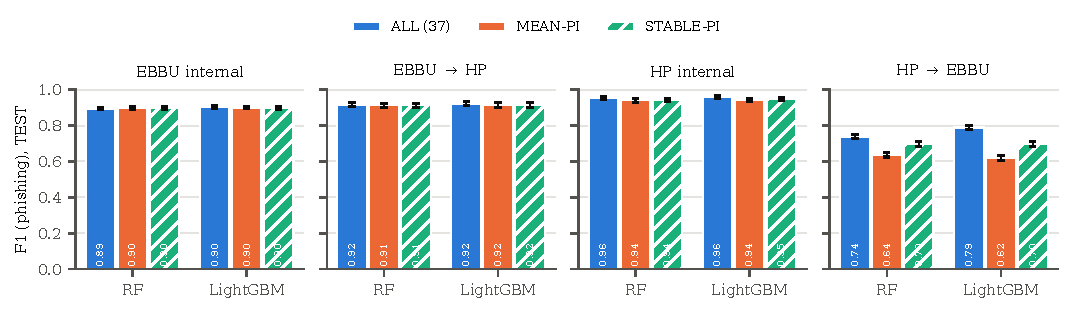
\includegraphics[width=\textwidth]{generated/fig_f1.pdf}
\caption{F1 on TEST for the four evaluation cells (bars: mean of 3 seeds; whiskers: 95\% domain-cluster bootstrap CI). Feature sets: ALL (blue), MEAN-PI (orange), STABLE-PI (green, hatched).}
\label{fig:f1}
\end{figure*}

\subsection{RQ2: stability-based versus mean-importance selection}
Table~\ref{tab:contrasts} lists the four pre-specified contrasts. In EBBU$\rightarrow$HP, differences between STABLE-PI and MEAN-PI are small (RF \res{DeltaABRF} [\res{DeltaLoABRF}, \res{DeltaHiABRF}], LightGBM \res{DeltaABLGBM} [\res{DeltaLoABLGBM}, \res{DeltaHiABLGBM}]) relative to the pre-set practical band. We do not claim statistical equivalence. In HP$\rightarrow$EBBU, the paired differences favour STABLE-PI: \res{DeltaBARF} [\res{DeltaLoBARF}, \res{DeltaHiBARF}] for RF and \res{DeltaBALGBM} [\res{DeltaLoBALGBM}, \res{DeltaHiBALGBM}] for LightGBM; the sign is positive in every seed, although the size varies (Table~\ref{tab:contrasts}). Internally, the observed selector differences are below the practical threshold.

The secondary contrasts temper this result: reduced subsets did not match ALL across both datasets. On HP$\rightarrow$EBBU, the STABLE-PI minus ALL F1 differences are \res{SecBARFSTABLEALL} (RF) and \res{SecBALGBMSTABLEALL} (LightGBM), while MEAN-PI minus ALL gives \res{SecBARFMEANALL} and \res{SecBALGBMMEANALL}. Stability ranking mitigates the loss associated with these compact configurations, without recovering ALL performance. This does not prove that the feature count alone causes the loss; membership and fitted trees also differ. On EBBU$\rightarrow$HP the STABLE-PI minus ALL differences are \res{SecABRFSTABLEALL} and \res{SecABLGBMSTABLEALL}.

\begin{table*}[t]
\caption{Paired domain-cluster bootstrap contrasts of target-TEST F1 (\res{nBoot} replicates; same resampled domains for both arms and all seeds). Top: the four primary contrasts; bottom: secondary cross-dataset contrasts. Per-seed deltas for seeds 17/29/43.}
\label{tab:contrasts}
\centering\scriptsize
\begin{tabular}{lllcccc}
\toprule
Cell & Model & Contrast & $k$ & $\Delta$F1 & 95\% CI & per seed \\
\midrule
A$\rightarrow$B & RF & STABLE vs MEAN (matched $k$) & 16/16/16 vs 16/16/16 & -0.000 & [-0.001, +0.000] & +0.000 +0.002 -0.004 \\
A$\rightarrow$B & LGBM & STABLE vs MEAN (matched $k$) & 16/16/16 vs 16/16/16 & -0.000 & [-0.001, +0.000] & +0.000 -0.002 +0.001 \\
B$\rightarrow$A & RF & STABLE vs MEAN (matched $k$) & 8/8/8 vs 8/8/8 & +0.059 & [+0.051, +0.066] & +0.095 +0.014 +0.066 \\
B$\rightarrow$A & LGBM & STABLE vs MEAN (matched $k$) & 8/8/8 vs 8/8/8 & +0.077 & [+0.069, +0.086] & +0.073 +0.039 +0.120 \\
\midrule
A$\rightarrow$B & RF & STABLE vs ALL & 16/16/16 vs 37/37/37 & -0.004 & [-0.006, -0.003] & -0.001 -0.002 -0.010 \\
A$\rightarrow$B & RF & MEAN vs ALL & 16/16/16 vs 37/37/37 & -0.004 & [-0.005, -0.002] & -0.001 -0.005 -0.006 \\
A$\rightarrow$B & RF & STABLE vs MEAN (budget $k$) & 16/16/16 vs 16/16/16 & -0.000 & [-0.001, +0.000] & +0.000 +0.002 -0.004 \\
A$\rightarrow$B & LGBM & STABLE vs ALL & 16/16/16 vs 37/37/37 & -0.007 & [-0.009, -0.004] & -0.007 -0.007 -0.006 \\
A$\rightarrow$B & LGBM & MEAN vs ALL & 16/16/16 vs 37/37/37 & -0.006 & [-0.009, -0.004] & -0.007 -0.005 -0.007 \\
A$\rightarrow$B & LGBM & STABLE vs MEAN (budget $k$) & 16/16/16 vs 16/16/16 & -0.000 & [-0.001, +0.000] & +0.000 -0.002 +0.001 \\
B$\rightarrow$A & RF & STABLE vs ALL & 8/8/8 vs 37/37/37 & -0.042 & [-0.050, -0.033] & -0.048 -0.027 -0.049 \\
B$\rightarrow$A & RF & MEAN vs ALL & 8/8/8 vs 37/37/37 & -0.100 & [-0.109, -0.092] & -0.143 -0.041 -0.116 \\
B$\rightarrow$A & RF & STABLE vs MEAN (budget $k$) & 8/8/8 vs 8/8/8 & +0.059 & [+0.051, +0.066] & +0.095 +0.014 +0.066 \\
B$\rightarrow$A & LGBM & STABLE vs ALL & 8/8/8 vs 37/37/37 & -0.093 & [-0.101, -0.085] & -0.093 -0.093 -0.093 \\
B$\rightarrow$A & LGBM & MEAN vs ALL & 8/8/8 vs 37/37/37 & -0.170 & [-0.181, -0.159] & -0.166 -0.132 -0.212 \\
B$\rightarrow$A & LGBM & STABLE vs MEAN (budget $k$) & 8/8/8 vs 8/8/8 & +0.077 & [+0.069, +0.086] & +0.073 +0.039 +0.120 \\
\bottomrule
\end{tabular}

\end{table*}

\subsection{RQ3: computational cost}
Table~\ref{tab:cost} and Fig.~\ref{fig:latency} give the latency per URL. For a single URL on one thread, reduced subsets take \res{relLatB1Min}--\res{relLatB1Max} of the end-to-end time of the corresponding ALL model; for batches of 1{,}024 URLs on four threads the ratio is \res{relLatBkMin}--\res{relLatBkMax}. Parsing and feature extraction account for a median of \res{extractShareMedian}\% of single-URL end-to-end time, so pruning features mainly saves extraction work, while tree inference cost depends little on the number of input features.

\begin{table*}[t]
\caption{Cost of the seed-17 model of every configuration (median $\mu$s per URL; ``rel.'' = end-to-end time relative to ALL of the same source and classifier). Hardware: \res{cpu}, \res{ram} GB RAM, Python \res{pyver}.}
\label{tab:cost}
\centering\scriptsize
\begin{tabular}{lllrrrrrrrrr}
\toprule
 & & & & \multicolumn{4}{c}{batch 1, 1 thread ($\mu$s/URL)} & \multicolumn{2}{c}{batch 1024, 4 thr.} & & \\
\cmidrule(lr){5-8}\cmidrule(lr){9-10}
Src & Model & Features & $k$ & extract & predict & e2e & rel. & e2e $\mu$s/URL & rel. & MB & fit s \\
\midrule
A & LGBM & MEAN-PI & 16 & 172 & 821 & 888 & 0.76 & 74.3 & 0.66 & 0.99 & 0.6 \\
A & LGBM & STABLE-PI & 16 & 177 & 598 & 881 & 0.75 & 75.0 & 0.67 & 0.99 & 0.6 \\
A & LGBM & ALL & 37 & 252 & 908 & 1167 & 1.00 & 112.5 & 1.00 & 1.00 & 0.8 \\
A & RF & MEAN-PI & 16 & 131 & 9881 & 9995 & 0.83 & 122.2 & 0.81 & 55.75 & 2.7 \\
A & RF & STABLE-PI & 16 & 112 & 9575 & 10110 & 0.84 & 121.0 & 0.81 & 55.75 & 2.7 \\
A & RF & ALL & 37 & 155 & 10244 & 12094 & 1.00 & 150.3 & 1.00 & 56.45 & 3.1 \\
B & LGBM & MEAN-PI & 8 & 150 & 539 & 772 & 0.93 & 61.0 & 0.55 & 0.99 & 0.6 \\
B & LGBM & STABLE-PI & 8 & 146 & 486 & 721 & 0.87 & 52.6 & 0.47 & 0.99 & 0.5 \\
B & LGBM & ALL & 37 & 228 & 556 & 830 & 1.00 & 111.3 & 1.00 & 1.00 & 0.9 \\
B & RF & MEAN-PI & 8 & 105 & 10316 & 10795 & 1.10 & 152.1 & 1.01 & 45.91 & 1.7 \\
B & RF & STABLE-PI & 8 & 111 & 10704 & 10455 & 1.06 & 92.7 & 0.61 & 44.15 & 1.5 \\
B & RF & ALL & 37 & 150 & 9356 & 9852 & 1.00 & 151.1 & 1.00 & 41.45 & 3.6 \\
\bottomrule
\end{tabular}

\end{table*}

\subsection{RQ4: attributions}
Some saved RF explanations exceed the additivity tolerance (maximum residual \res{shapAddErr}); the following rankings are diagnostic and must not be read as a complete validation of explanation fidelity.
SHAP rankings of the same model on source and target TEST samples agree to a Spearman $\rho$ of \res{rhoMin}--\res{rhoMax} (Table~\ref{tab:shap}, Fig.~\ref{fig:shap}); seed-to-seed agreement of the ALL models on the source is at least \res{rhoSeedMin}. Fig.~\ref{fig:pi} shows the permutation-importance evidence from which the subsets were drawn. Because the input distribution changes between cohorts, a different ranking on the target describes \emph{what} the model used there; it is not by itself evidence of an unfaithful explanation, nor of a causal role of a feature.

\begin{table*}[t]
\caption{SHAP rank agreement: source vs.\ target TEST ($\rho$, top-10 Jaccard) and across seeds for ALL; top-5 features on the source.}
\label{tab:shap}
\centering\scriptsize
\begin{tabular}{lllcccp{3.2cm}}
\toprule
Dir. & Model & Features & $\rho_{\mathrm{src,tgt}}$ & J$_{10}$ & $\rho_{\mathrm{seeds}}$ & top-5 (source) \\
\midrule
A$\rightarrow$B & LGBM & ALL (37) & 0.99 & 0.82 & 1.00 & \scriptsize F23 F09 F30 F06 F03 \\
A$\rightarrow$B & LGBM & STABLE-PI & 0.88 & 0.82 & -- & \scriptsize F23 F09 F03 F06 F30 \\
A$\rightarrow$B & RF & ALL (37) & 0.97 & 0.82 & 1.00 & \scriptsize F23 F09 F30 F07 F03 \\
A$\rightarrow$B & RF & STABLE-PI & 0.81 & 0.82 & -- & \scriptsize F23 F09 F03 F30 F07 \\
B$\rightarrow$A & LGBM & ALL (37) & 0.96 & 0.82 & 1.00 & \scriptsize F02 F23 F06 F03 F22 \\
B$\rightarrow$A & LGBM & STABLE-PI & 0.98 & 1.00 & -- & \scriptsize F02 F23 F03 F06 F21 \\
B$\rightarrow$A & RF & ALL (37) & 0.95 & 0.82 & 1.00 & \scriptsize F02 F23 F06 F01 F03 \\
B$\rightarrow$A & RF & STABLE-PI & 0.98 & 1.00 & -- & \scriptsize F02 F23 F06 F03 F21 \\
\bottomrule
\end{tabular}

\end{table*}

\begin{figure*}[t]
\centering
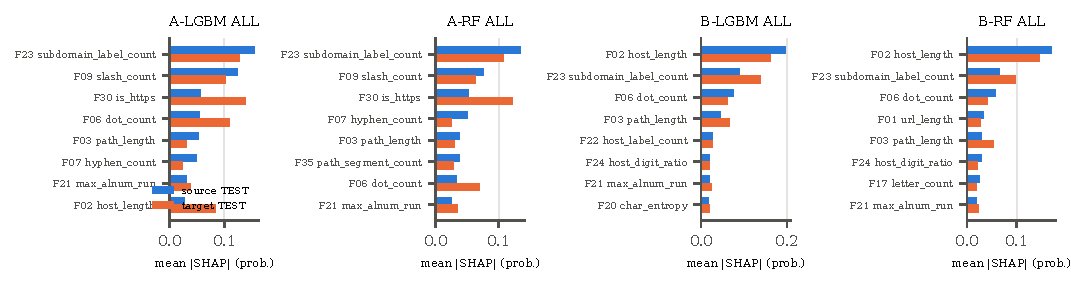
\includegraphics[width=\textwidth]{generated/fig_shap.pdf}
\caption{Mean $|$SHAP$|$ (probability scale) of the eight most important features of the seed-17 ALL models on source TEST (blue) and target TEST (orange).}
\label{fig:shap}
\end{figure*}

\begin{figure*}[t]
\centering
\begin{minipage}[t]{0.48\textwidth}
\centering\vspace{0pt}
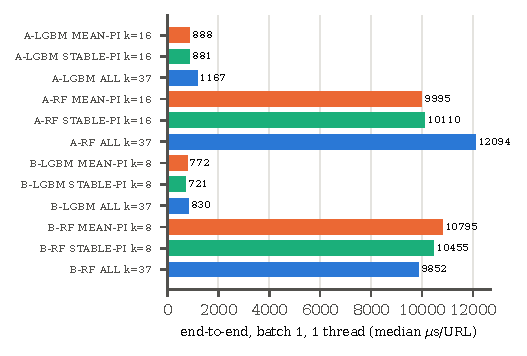
\includegraphics[width=\linewidth]{generated/fig_latency.pdf}
\caption{End-to-end latency for a single URL on one thread (seed-17 models).}
\label{fig:latency}
\end{minipage}\hfill
\begin{minipage}[t]{0.48\textwidth}
\centering\vspace{0pt}
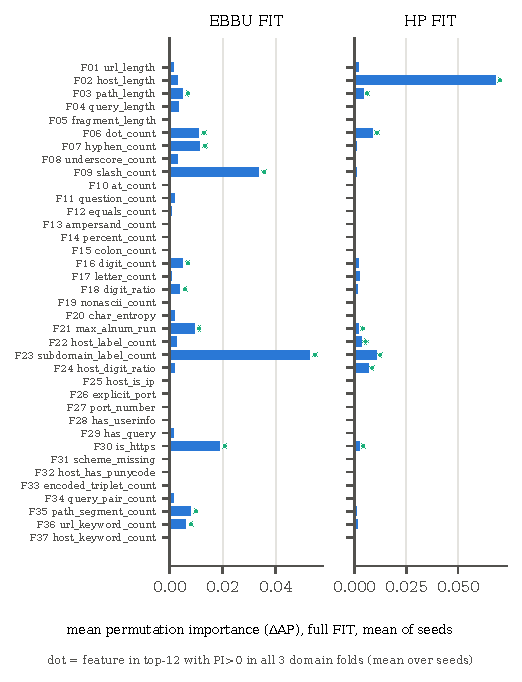
\includegraphics[width=\linewidth]{generated/fig_pi.pdf}
\caption{Permutation importance on full FIT (mean over folds and seeds). Dots mark features that are in the top 12 with positive PI in all three domain folds.}
\label{fig:pi}
\end{minipage}
\end{figure*}

\section{Discussion}
\textit{Interpreting transfer asymmetry.} The FIT partitions show descriptive source differences: HP benign URLs are short (median \res{medLenBBenign} characters) and mostly HTTPS (\res{httpsBBenign}\%), whereas HP phishing URLs are longer (\res{medLenBPhish}) with more dots and subdomains (medians \res{medDotsBPhish} and \res{medSubBPhish}). In EBBU, phishing URLs have medians of \res{medSubAPhish} subdomains and \res{medDotsAPhish} dots and are rarely HTTPS (\res{httpsAPhish}\%), but neither are its benign URLs (\res{httpsABenign}\% HTTPS). These differences are consistent with collection-specific cues contributing to the observed asymmetry; they do not establish which feature caused an error. Rashid~\textit{et al.}~\cite{rashid2024} already discuss feature-distribution differences, so identifying source shift is not our novelty. The two datasets differ in collection process, period and prevalence; our transfer drop describes this benchmark pair rather than isolating a causal domain-shift effect.

\textit{What does stability buy?} STABLE-PI prioritises features with more positive top-$q$ fold votes; it does not require every selected feature to be stable in all folds and does not guarantee invariance across datasets. It outperformed mean ranking at the same small budget in HP$\rightarrow$EBBU, without a clear advantage in the other direction. The matched-$k$ design separates this ranking comparison from the number of retained features. ALL nevertheless remained the stronger cross-dataset reference. Our empirical insight is therefore conditional: source-domain stability can mitigate the loss from a compact subset in this benchmark, but it does not establish that source-selected compression preserves transfer or that the rule is generally safer.

\textit{What the two-paper extension establishes.} We connect the classifier/representativeness questions in~\cite{sanchez2022} with the transfer problem in~\cite{rashid2024} through a controlled source-only evaluation. Both primary papers satisfy the five-year recency limit; original EBBU provenance is retained in the repository. The contribution lies in the auditable protocol and the ranking--budget--cost comparison. We have not run either original system under identical conditions, so we cannot attribute improvements over their published results to our approach. The two primary papers satisfy the revised project count and recency conditions; they do not establish universal novelty, and relevant adjacent work remains acknowledged.

\textit{Uncertainty.} The bootstrap intervals resample target domains for fixed fitted models; they do not include resampling or split-induced training variability. Table~\ref{tab:contrasts} shows that per-seed differences vary, so the size of the advantage is less stable than its observed sign. Three estimator seeds on a single split do not establish a population-level training effect, and we make no family-wise significance claim. Additional independently collected holdout data and repeated training splits would strengthen robustness claims, but must be planned under a new protocol before opening a new holdout.

\textit{Cost.} Lexical models are already cheap; reducing 37 to 8--16 features trims extraction work but the shared parsing step and the per-call overhead of the model remain, so savings are modest relative to the accuracy given up on the hard direction. ``Lightweight'' is therefore relative to the ALL model on the reported hardware.

\textit{Threats to validity.} (i) Both datasets are older public collections; results do not establish contemporary or zero-day robustness. (ii) The symmetric purge removes shared popular domains and changes the evaluation population. (iii) Both selectors share an RF proxy, which may favour RF. (iv) Correlated lexical features can depress PI. (v) Hyper-parameters were fixed, not optimised. (vi) Numeric HP label encoding was verified indirectly through the repository's copy of EBBU; complete primary-paper checks remain pending. (vii) The freeze is a procedural control, signed by an agent on the author's instruction. (viii) Some saved SHAP outputs fail the additivity tolerance, so attributions cannot substantiate causal or fully validated explanation claims. The notebook audit also identified direct TEST-vault access in the frozen legacy SHAP analysis; the repaired notebook does not execute that path, but a corrected analysis must follow the versioning rules.

\section{Conclusion}
On a domain-disjoint EBBU/HP benchmark with a frozen, source-only learning protocol, lexical URL classifiers transferred well from EBBU to HP (F1 \res{F1ABLGBMALL} for LightGBM) but lost \res{DropBLGBMALL}--\res{DropBRFALL} F1 points from HP to EBBU (RQ1). Stability ranking gave higher target F1 than mean ranking at the same budget in the harder direction (\res{DeltaBARF} RF, \res{DeltaBALGBM} LightGBM), without a clear advantage in the other direction; reduced subsets did not match the full feature set across datasets (RQ2). Latency trade-offs depend on the model and execution setting (RQ3). SHAP comparisons remain diagnostic because some saved outputs fail additivity validation (RQ4). The contribution is a reproducible empirical comparison under a defined target-access constraint, not a new classifier or a demonstrated improvement over UDA. Future work should resolve explanation validation, evaluate more recent independent sources, and quantify training variability with repeated splits under a new protocol before opening a new holdout.

\section*{Data and Code Availability}
Raw data are not redistributed (licences unclear); the package downloads EBBU (\texttt{ebubekirbbr/pdd@90b394d}) and HP (\texttt{fariza25/PhishingURLDetection@ff9f1f5}) at pinned commits and verifies SHA256 hashes. Code, configuration, lockfile, schemas, decision log and the freeze manifest (\texttt{\res{freezeHash}}) are in the project repository; every number in this paper is generated by \texttt{phishresearch.cli report}.


\bibliographystyle{IEEEtran}
\bibliography{refs}

\end{document}
